%% ------------------------------------------------------------ %%
\chapter{Diagnóstico Bayesiano em Modelos de Regressão Simétricos}
\label{cap:simetrico}

O modelo de regressão Normal é um dos modelos mais conhecidos e utilizados, porém sua versatilidade costuma ser superestimada. Uma das fragilidades deste modelo está na hipótese de normalidade dos erros. Uma das características da distribuição Normal, além da sua simetria, é o baixo peso de suas caudas. Assim, sob a suposição de normalidade observações distantes da média possuem baixa probabilidade de ocorrência e, quando essas observações aparecem na amostra, acabam por influenciar muito as estimativas deste modelo. 

Uma possível solução para anular a influência de observações discrepantes (muito distantes da média) nas estimativas do modelo seria deletá-las. Porém, não é óbvio decidir quais observações deveriam ser deletadas já que não existe um único critério para classificar uma observação como discrepante. Uma solução melhor é propor um modelo que seja menos influenciado por observações discrepantes, mas que não despreze completamente estas observações.

O modelo de regressão com erros com distribuição $t$-Student tem sido proposto como um modelo mais robusto que o normal, isto é, menos influenciado por observações discrepante, devido ao fato de possuir caudas mais pesadas que a distribuição normal. No entanto, a obtenção das estimativas dos parâmetros do modelo $t$-Student apresenta dificuldades que não são encontradas no modelo normal. Sob o paradigma bayesiano, essas estimativas dependem da obtenção da distribuição \textit{a posteriori} dos parâmetros de interesse e, neste caso, técnicas computacionais são necessárias.

Sob qualquer um destes modelos ainda precisamos conseguir identificar de uma forma precisa quais observações são discrepantes já que uma análise visual pode ser arbitrária. Também precisamos, uma vez identificadas tais observações, saber se estas são de fato influentes nas estimativas dos parâmetros do modelo. Uma medida utilizada para identificação de pontos discrepantes é a \textit{conditional predictive ordinate} (CPO). Neste capítulo mostramos o cálculo dessa estatística para os modelos de regressão linear normal e $t$-Student. A influência das observações nas estimativas é abordada por meio das medidas de divergência norma $L_1$ e Kullback-Leibler. Tais medidas de influência são calculadas tanto para os parâmetros dos modelos de uma forma global, isto é, para o conjunto completo de parâmetros do modelo; quanto marginalmente, apenas para os coeficientes regressores.

Ao final do capítulo, aplicamos ambos os modelos a um conjunto de dados presente em \citet{WeissCho1998} e utilizado em outros trabalhos que tratam de pontos discrepantes. Além de aplicar os modelos, também mostramos como estes são influenciados pelas observações. 

%% ------------------------------------------------------------ %%
\section{Medidas de Diagnóstico}

Uma técnica estatística amplamente utilizada para avaliar a qualidade de um determinado modelo é a validação cruzada. Esta técnica tem como objetivo avaliar a capacidade de previsão de um modelo estatístico a partir de um conjunto de dados fixado. Assim, particiona-se o conjunto de dados em duas partes. A primeira parte, denominada amostra de treinamento, é utilizada para obter as estimativas dos parâmetros do modelo proposto e a segunda, denominada amostra de validação, é utilizada para verificar a qualidade das estimativas deste modelo frente a novos dados.

Considere, inicialmente, $\ybf=(y_1,\ldots,y_n)$ uma amostra aleatória simples observada de um modelo $Y|\theta$. Sejam $I_1,\ldots,I_K$ tais que $\{1,\ldots,n\} = \cup_{k = 1}^K I_k$ e, $\forall i\neq j$, $I_i\cap I_j=\varnothing$, isto é, $I_1,\ldots,I_K$ é uma partição do conjunto de índices $\{1,\ldots,n\}$. O processo da validação cruzada consiste em $K$ etapas de estimação de parâmetros e validação destas estimativas.  Na $k$-ésima etapa separamos nossos dados em dois conjuntos: $\ybf_{(I_k)}=(y_j)_{j\notin I_k}$ e $\ybf_{I_k}=(y_j)_{j\in I_k}$. Dessa forma, utilizamos o primeiro conjunto, $\ybf_{(I_k)}$, para obter uma estimativa de $\theta$ e o segundo conjunto, $\ybf_{I_k}$, para validação desta estimativa. Após as $K$ etapas, todas as observações foram utilizadas para validar estimativas das quais elas não fizeram parte. Usualmente, os conjuntos $I_k$ possuem o mesmo tamanho e são escolhidos de forma aleatória. Existem diversos procedimentos para se conduzir tal processo de validação cruzada sendo o método \textit{leave-one-out} um dos mais comuns.

O método \textit{leave-one-out} considera $K=n$ e assim teremos $I_i=\{i\}$, para cada $i=1,\ldots,n$. Dessa forma, vamos obter a estimativa de $\theta$ em $\yi = (y_j)_{j\neq i}$ e validar na observação $y_i$. A distribuição preditiva de $\yi$ dada por
\begin{equation}\label{eq:pred_cpo}
f(y_i|\yi) = \int  f(y_i|\theta)f(\theta|\yi) d\theta
\end{equation}
é a densidade da amostra de validação, neste caso composta por somente $y_i$, dado o restante dos dados, $\yi$. A quantidade $f(y_i|\yi)$ é chamada de $i$-ésima ordenada preditiva condicional, em inglês \textit{conditional predictive ordinate} ($CPO_i$). Portanto, valores baixos de $CPO_i$ podem ser associados a valores discrepantes sob o modelo proposto, já que a densidade calculada no ponto $y_i$ indicará uma região de baixa probabilidade. Uma maneira de comparar a falta de adequação de cada observação em diferentes modelos propostos é por meio da comparação das $CPO_i$ calculadas sob cada modelo. Perceba que tal comparação é possível pois, como podemos ver na equação \eqref{eq:pred_cpo}, o $CPO_i$ é uma medida que depende somente da distribuição preditiva pois todos os parâmetros são integrados.

Note que podemos escrever
\begin{equation}\label{eq:cpo_first}
f(y_i|\yi) = \int f(y_i|\yi,\theta)f(\theta|\yi) d\theta = \int f(y_i|\theta)f(\theta|\yi) d\theta = E_{\theta|\yi}[f(y_i|\theta)]
\end{equation}
e, sendo $\theta^{(1)},\ldots,\theta^{(L)}$ uma amostra de tamanho $L$ da distribuição \textit{a posteriori} de $\theta|\yi$, por meio da integração de Monte Carlo, podemos aproximar \eqref{eq:cpo_first} por

\begin{equation}\label{eq:cpo_approx}
 E_{\theta|\yi}[f(y_i|\theta)]\approx \frac{1}{L}\sum_{l=1}^L f(y_i|\theta^{(l)}).
\end{equation}

Porém, a aproximação apresentada em \eqref{eq:cpo_approx} necessita a obtenção de uma amostra da distribuição \textit{a posteriori} de $\theta|\yi$ para cada $i=1,\ldots,n$ e isto pode ser computacionalmente muito custoso. Podemos utilizar a seguinte caracterização alternativa para o $CPO_i$, que simplifica o esforço computacional pois a esperança é calculada com a distribuição \textit{a posteriori} completa de $\theta|\ybf$ para todo $i=1,\ldots,n$
\begin{equation}\label{eq:cpo_final}
\begin{split}
f(y_i|\yi) & = \frac{f(\ybf)}{f(\yi)} = \frac{\int f(\ybf|\theta) f(\theta) d\theta}{\int f(\yi|\theta) f(\theta) d\theta} = \frac{\int \frac{f(\ybf|\theta) f(\theta)}{f(\ybf)} d\theta}{\int \frac{f(\yi|\theta) f(\theta)}{f(\ybf)} \frac{f(\theta|\ybf)}{f(\theta|\ybf)} d\theta} \\
{}& = \frac{\int f(\theta|\ybf) d\theta}{\int \frac{f(\yi|\theta) f(\theta)}{f(\ybf)} \frac{f(\ybf)}{f(\ybf|\theta)f(\theta)} f(\theta|\ybf) d\theta} = \frac{1}{\int \frac{1}{f(y_i|\theta)} f(\theta|\ybf) d\theta} \\
{} & = E_{\theta|\ybf}[f(y_i|\theta)^{-1}]^{-1}
\end{split}
\end{equation}
e a equação \eqref{eq:cpo_final} pode ser aproximada por
\begin{equation}\label{eq:cpo_final_mc}
E_{\theta|\ybf}[f(y_i|\theta)^{-1}]^{-1} \approx \left(\frac{1}{L}\sum_{l=1}^L\frac{1}{f(y_i|\theta^{(l)})}\right)^{-1},
\end{equation}
onde $\theta^{(1)},\ldots,\theta^{(L)}$ é uma amostra de tamanho $L$ de $\theta|\ybf$ em que $\ybf$ é o vetor com todas as observações. Agora, precisamos de somente uma amostra da distribuição \textit{a posteriori} completa para o cálculo do $CPO_i$.

Uma medida resumo natural para os $CPO_i$ é a \textit{log pseudo marginal likelihood} (LMPL), sugerida em \citet{Ibrahim2001}, definida por
\begin{equation}
LPML = \sum_{i=1}^n\log(CPO_i).
\end{equation}
Essa estatística pode ser considerada uma medida de ajuste. O modelo que possuir o maior valor de LPML será considerado o mais adequado aos dados.

Utilizaremos o $CPO_i$ para identificar observações discrepantes. Mais precisamente, utilizaremos a estatística $-\log(CPO_i)$ pois as observações discrepantes ficam mais evidentes em uma inspeção gráfica.

\subsection{Influência Global}

Uma medida de influência de cada observação na estimação de um vetor de parâmetros $\theta$ é dada pela divergência entre a distribuição \textit{a posteriori} $f(\theta|\ybf)$ e a distribuição \textit{a posteriori} obtida na ausência da $i$-ésima observação $f(\theta|\yi)$. A família de divergências apresentada em \citet{Weiss1996} é dada por
\begin{equation}\label{eq:def_div}
D_\theta(g,i)=\int g\left(\frac{f(\theta|\yi)}{f(\theta|\ybf)}\right)f(\theta|\ybf) d\theta,
\end{equation}
onde $g$ é uma função convexa com $g(1)=0$.

Sob a ausência de influência da $i$-ésima observação, teríamos que $f(\theta|\ybf)=f(\theta|\yi)$ e assim
\begin{equation}
D_\theta(g,i)=\int g\left(\frac{f(\theta|\ybf)}{f(\theta|\ybf)}\right)f(\theta|\ybf) d\theta =\int g(1)f(\theta|\ybf) d\theta =  0.
\end{equation}

Note também que $D_\theta(g,i) \geqslant 0$ pois, sendo $g$ convexa, pela desigualdade de Jensen,
\begin{equation}
\begin{split}
D_\theta(g,i)&=\int g\left(\frac{f(\theta|\yi)}{f(\theta|\ybf)}\right)f(\theta|\ybf) d\theta = E_{\theta|\ybf}\left[g\left(\frac{f(\theta|\yi)}{f(\theta|\ybf)}\right)\right] \\
{} & \geqslant g\left(E_{\theta|\ybf}\left[\frac{f(\theta|\yi)}{f(\theta|\ybf)}\right]\right) = g\left(\int f(\theta|\yi)d\theta\right) = g(1) =0.
\end{split}
\end{equation}

Teremos que, se $g$ for estritamente convexa em $1$, $D_\theta(g,i) = 0$ se, e somente se, $f(\theta|\ybf)=f(\theta|\yi)$ quase certamente. Logo, a divergência $D_\theta(g,i)$ nos dará uma medida de dissimilaridade entre as distribuições $f(\theta|\ybf)$ e $f(\theta|\yi)$.

A $CPO_i$, definida anteriormente, é relacionada com a divergência da seguinte forma
\begin{equation}
\frac{f(\theta|\yi)}{f(\theta|\ybf)} = \frac{\frac{f(\yi|\theta)f(\theta)}{f(\yi)}}{\frac{f(\ybf|\theta)f(\theta)}{f(\ybf)}} = \frac{f(\yi|\theta)}{f(\ybf|\theta)}\frac{f(\ybf)}{f(\yi)}=\frac{1}{f(y_i|\theta)}f(y_i|\yi) = \frac{CPO_i}{f(y_i|\theta)} = h_i(\theta)
\end{equation}
e usualmente $h_i$ é chamada de função de perturbação.

Portanto,
\begin{equation}
D_\theta(g,i)=\int g\left(\frac{f(\theta|\yi)}{f(\theta|\ybf)}\right)f(\theta|\ybf) d\theta = E_{\theta|\ybf}\left[g\left(\frac{f(\theta|\yi)}{f(\theta|\ybf)}\right)\right]= E_{\theta|\ybf}\left[g\left(\frac{CPO_i}{f(y_i|\theta)}\right)\right].
\end{equation}

Uma forma aproximada de obter $D_\theta(g,i)$ é por meio da integração de Monte Carlo. Seja $\theta^{(1)},\ldots,\theta^{(L)}$, uma amostra simulada de tamanho $L$ da distribuição \textit{a posteriori} de $\theta|\ybf$, podemos obter a seguinte aproximação
\begin{equation}\label{eq:div_glo_final}
D_\theta(g,i)\approx \frac{1}{L}\sum_{l=1}^ng\left(\frac{CPO_i}{f(y_i|\theta^{(l)})}\right),
\end{equation}
a qual é fácil de ser calculada pois já vimos na equação \eqref{eq:cpo_final_mc} como obter uma estimativa do $CPO_i$ e $f(y_i|\theta)$ sempre terá uma forma conhecida. Caso tentássemos trabalhar com a primeira representação de $D_\theta(g,i)$ apresentada na equação \eqref{eq:def_div}, precisaríamos obter formas explícitas para $f(\theta|\ybf)$ e $f(\theta|\yi)$ e isto nem sempre é possível de obter.

Neste trabalho vamos nos restringir a duas medidas específicas de divergência: norma $L_1$ e divergência de Kullback-Leibler.

\subsubsection{Norma $L_1$}
A norma $L_1$ é um caso particular da divergência apresentada na equação \eqref{eq:def_div} com $g(a) = \frac{1}{2}|a-1|$. Para que $g$ seja uma função que define uma divergência precisamos que $g(1)=0$ e que $g$ seja convexa. A primeira condição é satisfeita de forma clara. Para verificar a convexidade, seja $a_1,a_2\in \mathbb{R}$ e $\alpha\in [0,1]$, então

\begin{equation}
\begin{split}
g(\alpha a_1+(1-\alpha)a_2) &= \frac{1}{2}|\alpha a_1+(1-\alpha)a_2-1| = \frac{1}{2}|\alpha(a_1-1)+(1-\alpha)(a_2-1)| \\
{} & \leqslant \alpha\frac{1}{2}|a_1-1|+(1-\alpha)\frac{1}{2}|a_2-1| = \alpha g(a_1) + (1-\alpha)g(a_2).
\end{split}
\end{equation}

A norma $L_1$ será dada por
\begin{equation}
\begin{split}
L_{1i,\theta} &= D_\theta(g,i)=\int g\left(\frac{f(\theta|\yi)}{f(\theta|\ybf)}\right)f(\theta|\ybf) d\theta = \int \frac{1}{2}\left|\frac{f(\theta|\yi)}{f(\theta|\ybf)}-1\right|f(\theta|\ybf) d\theta \\
{}& = \frac{1}{2} \int |f(\theta|\yi)-f(\theta|\ybf)| d\theta.
\end{split}
\end{equation}

Uma caracterização alternativa para norma $L_1$ é
\begin{equation}\label{eq:l1_alt}
L_{1i,\theta} = \sup_B \int_B \left( f(\theta|\yi) - f(\theta|\ybf) \right) d\theta = \sup_B \int_B \left( f(\theta|\ybf) - f(\theta|\yi) \right) d\theta.
\end{equation}
A caracterização apresentada em \eqref{eq:l1_alt} é conhecida como distância variacional total. Podemos interpretá-la como a maior diferença possível entre as funções densidade $f(\theta|\ybf)$ e $f(\theta|\yi)$. Como \citet{Weiss1996} observa, na equação \eqref{eq:l1_alt} o supremo da primeira igualdade é atingido no conjunto $B=\{\theta: f(\theta|\yi)>f(\theta|\ybf)\}$ enquanto que o supremo da segunda igualdade é atingido no conjunto complementar de $B$.

Como, para todo $x,y\in \mathbb{R}$, vale que $|x-y|\leqslant |x|+|y|$, teremos que $L_{1i,\theta}\leqslant 1$ pois
\begin{equation}
\begin{split}
L_{1i,\theta} &= \frac{1}{2} \int |f(\theta|\yi)-f(\theta|\ybf)| d\theta \leqslant \frac{1}{2} \int \left(f(\theta|\yi)+f(\theta|\ybf)\right) d\theta \\
{}& = \frac{1}{2} \int f(\theta|\yi)d\theta + \frac{1}{2} \int f(\theta|\ybf) d\theta = 1
\end{split}
\end{equation}

Logo, podemos ver que na função $g$ a constante $\frac{1}{2}$ faz com que o valor máximo de $L_{1i,\theta}$ seja $1$.

\subsubsection{Kullback-Leibler}

A divergência de Kullback-Leibler é o caso particular de \eqref{eq:def_div} quando $g(a)=a\log(a)$, com $a>0$. Veja que também claramente $g(1)=0$. Para verificar a convexidade, note que
\begin{equation}
g'(a)=\log(a)+1 \Rightarrow g''(a)=\frac{1}{a} > 0.
\end{equation}
Logo, sendo a segunda derivada positiva para todo $a>0$, $g$ é convexa.

A divergência de Kullback-Leibler fica dada por 
\begin{equation}
\begin{split}
K_{i,\theta} &= D_\theta(g,i)=\int g\left(\frac{f(\theta|\yi)}{f(\theta|\ybf)}\right)f(\theta|\ybf) d\theta \\
{}  &=\int \frac{f(\theta|\yi)}{f(\theta|\ybf)}\log\left(\frac{f(\theta|\yi)}{f(\theta|\ybf)}\right)f(\theta|\ybf) d\theta \\
{}&= E_{\theta|\yi}[\log(f(\theta|\yi))]-E_{\theta|\yi}[\log(f(\theta|\ybf))]
\end{split}
\end{equation}

Não é possível encontrar de uma forma simples um limite superior para divergência de Kullback-Leibler como fizemos com a norma $L_1$. Além disso, ela é de difícil interpretação dificultando assim entender o que o seu valor representa. Há uma grande quantidade de trabalhos focados em dar uma interpretação a esta divergência. Contudo, podemos utilizar outras medidas de divergência que são intrinsecamente mais interpretáveis como, por exemplo, a norma $L_1$. 

\subsection{Influência Marginal}

Nem sempre estamos interessados na influência de uma observação no vetor completo de parâmetros $\theta$. Nosso interesse pode estar na influência de uma observação em parte do vetor, ou seja, estamos interessados em uma influência marginal. Denotando por $\theta=(\theta_1,\theta_2)$ o vetor completo de parâmetros, uma medida para influência da $i$-ésima observação nas estimativas de $\theta_1$ é dada pela divergência 
\begin{equation}
D_{\theta_1}(g,i) = \int g\left(\frac{f(\theta_1|\yi)}{f(\theta_1|\ybf)}\right) f(\theta_1|\ybf) d\theta_1
\end{equation}
que possui a definição análoga ao caso global.

Note que 
\begin{equation}
\frac{f(\theta_1|\yi)}{f(\theta_1|\ybf)} = \frac{\frac{f(\yi|\theta_1)f(\theta_1)}{f(\yi)}}{\frac{f(\ybf|\theta_1)f(\theta_1)}{f(\ybf)}} = \frac{f(\ybf)}{f(\yi)}\frac{1}{\frac{f(\ybf|\theta_1)}{f(\yi|\theta_1)}} = \frac{CPO_i}{f(y_i|\theta_1,\yi)}=h_{1i}(\theta_1)
\end{equation}
sendo $h_{1i}$ a função de perturbação neste caso marginal.

A medida de influência no vetor completo de parâmetros será maior do que em um subconjunto do vetor de parâmetros. Supondo $\theta=(\theta_1,\theta_2)$, o Teorema 2, p. 742, de \citet{Weiss1996} diz que
\begin{equation}
0\leqslant D_{\theta_1}(g,i)\leqslant D_\theta(g,i)
\end{equation}
Logo, a influência marginal será sempre menor ou igual que a influência global. Portanto, uma observação pode exercer influência de forma global, mas não de forma marginal no parâmetro de interesse.

Para encontrar um cálculo aproximado para $D_{\theta_1}(g,i)$, também utilizaremos a integração de Monte Carlo. Veja que precisamos encontrar o valor de $CPO_i$ e, a princípio, uma forma explícita para $f(y_i|\theta_1,\yi)$. Diferentemente do que ocorre no cálculo da divergência global onde $f(y_i|\theta)$ está sempre disponível, no cálculo da divergência marginal precisamos da quantidade $f(y_i|\theta_1,\yi)$ que nem sempre será fácil encontrar de forma explícita. A relação desenvolvida a seguir facilitará a obtenção de uma estimativa para essa distribuição. Note que,
\begin{equation}\label{eq:fyi_perturb}
\begin{split}
f(y_i|\theta_1,\yi) & = \int f(y_i|\theta)f(\theta_2|\theta_1, \yi) d \theta_2 = \int f(y_i|\theta)\frac{f(\theta,\yi)}{f(\theta_1,\yi)}d\theta_2 \\
{} & = \int f(y_i|\theta)\frac{f(\yi|\theta)f(\theta)}{f(\theta_1,\yi)}d\theta_2 = \int \frac{f(\ybf|\theta)f(\theta)}{f(\theta_1,\yi)}d\theta_2 \\
{} & \propto \int f(\ybf|\theta)f(\theta)d\theta_2
\end{split}
\end{equation}

Assim, encontramos uma forma proporcional para $f(y_i|\theta_1,\yi)$, mas precisamos ainda encontrar a constante de padronização integrando o último termo de \eqref{eq:fyi_perturb} em $y_i$.

A seguir apresentamos os modelos de regressão linear normal e $t$-Student e derivamos as medidas de diagnóstico aqui apresentadas para cada um dos modelos.

%% fim de seção------------------------------------------------- %%

\section{Modelo de Regressão Normal}
\label{sec:reg_Normal}

\subsection{Estimação dos Parâmetros}

O modelo de regressão linear com erros de distribuição normal é dado por
\begin{equation}
y_i = x_i^\transp\betabf + \epsilon_i,
\end{equation}
onde, para cada $i=1,\ldots,n$, $y_i$ é a variável resposta da $i$-ésima observação, $x_i^\transp=(1,x_{i1},\ldots,x_{ip})$ é o vetor de variáveis explicativas, $\betabf=(\beta_0,\beta_1,\ldots,\beta_p)^\transp$ é vetor de parâmetros desconhecidos a serem estimados e $\epsilon_i\sim N(0,\sigsq)$ independentes, ou seja, os erros possuem distribuição normal com média $0$ variância $\sigsq$.

Para cada $i$ temos que $y_i|\betabf,\sigsq \sim N(x_i^\transp\betabf,\sigma^2)$ e pela independência a verossimilhança deste modelo fica dada por
\begin{equation}
\begin{split}
L(\betabf,\sigsq) &=f(\ybf|\betabf,\sigsq)=\prod_{j=1}^nf(y_j|\betabf,\sigsq) =  \prod_{j=1}^n \frac{1}{\sqrt{2\pi\sigsq}}\exp\left(-\frac{(y_j-x_j^\transp\betabf)^2}{2\sigsq}\right) \\
{} & = \left(\frac{1}{\sqrt{2\pi\sigsq}}\right)^n\exp\left(-\frac{1}{2\sigsq}\sum_{j=1}^n (y_j-x_j^\transp\betabf)^2\right).
\end{split}
\end{equation}

Trataremos este e os outros modelos sob a perspectiva bayesiana de inferência, então é necessário também especificar distribuições \textit{a priori} para $\betabf$ e $\sigsq$. Neste estudo iremos usar distribuições \textit{a priori} não informativas considerando, assim, desconhecimento prévio a respeito dos parâmetros a serem estimados. 

A distribuição \textit{a priori} de Jeffreys é uma das mais utilizadas quando se quer trabalhar com distribuições \textit{a priori} não informativas e é definida por
\begin{equation}
f(\theta)\propto \sqrt{\det I(\theta)},
\end{equation}
onde $I(\theta)$ é a matriz de informação de Fisher de $\theta$ (ver \citet{Paulino2003}, página 99). Esta distribuição \textit{a priori} possui a propriedade básica de ser invariante sob reparametrizações.

Supondo independência \textit{a priori} entre $\betabf$ e $\sigsq$, e obtendo a distribuição \textit{a priori} de Jeffreys para cada parâmetro, teremos a seguinte distribuição \textit{a priori} conjunta
\begin{equation}\label{eq:Normal_prior}
f(\betabf,\sigsq)\propto \frac{1}{\sigsq}.
\end{equation}
A distribuição \textit{a posteriori} dos parâmetros do modelo de regressão fica dada por

\begin{align}
f(\betabf,\sigsq|\ybf)& \propto L(\betabf,\sigsq)f(\betabf,\sigsq) \notag \\
{}& \propto \left(\frac{1}{\sqrt{2\pi\sigsq}}\right)^n\exp\left(-\frac{1}{2\sigsq}\sum_{j=1}^n (y_j-x_j^\transp\betabf)^2\right) \frac{1}{\sigsq} \\
{}& \propto \frac{1}{\sigma^{n+2}}\exp\left(-\frac{1}{2\sigsq}\sum_{j=1}^n (y_j-x_j^\transp\betabf)^2\right) \notag 
\end{align}

e este é o núcleo de uma distribuição Normal-Gama Invertida. Podemos representar tal distribuição da forma hierárquica a seguir
\begin{equation}
\begin{split}
\betabf | \sigsq, \ybf & \sim N_{p+1}(\bhat,\sigsq(X^\transp X)^{-1})\\
\sigsq| \ybf & \sim GI\left(\frac{n-(p+1)}{2},\frac{(\ybf-X\bhat)^\transp(\ybf-X\bhat)}{2}\right),\\
\end{split}
\end{equation}
onde $\bhat = (X^\transp X)^{-1}X^\transp\ybf$ (ver \citet{Paulino2003}, página 211).

Uma forma de obter uma amostra de tamanho $L$ da distribuição \textit{a posteriori} conjunta de $(\betabf,\sigsq)|\ybf$ é utilizar o algoritmo a seguir: 
\begin{enumerate}
\item[] Para cada $l=1,\ldots,L$
\begin{enumerate}
\item Simular ${\sigsq}^{(l)}$ da distribuição de $\sigsq|\ybf$.
\item Simular $\betabf^{(l)}$ da distribuição de $\betabf|{\sigsq}^{(l)},\ybf$.
\end{enumerate}
\item[] Assim, $(\betabf^{(1)},{\sigsq}^{(1)}),\ldots,(\betabf^{(L)},{\sigsq}^{(L)})$ é a amostra desejada
\end{enumerate}

\subsection{Derivação das Medidas de Diagnóstico}

Considere $(\betabf^{(1)},{\sigsq}^{(1)}),\ldots,(\betabf^{(L)},{\sigsq}^{(L)})$ uma amostra de tamanho $L$ da distribuição \textit{a posteriori} de $\betabf,\sigsq|\ybf$. Utilizaremos esta amostra em todos os cálculos das medidas de diagnóstico.

Mostramos na equação \eqref{eq:cpo_final} como obter uma estimativa para o $CPO_i$ em um caso geral. No caso da regressão linear normal teremos
\begin{equation}\label{eq:cpo_est_norm}
\widehat{CPO_i} = \left[\frac{1}{L}\sum_{l=1}^L\frac{1}{f(y_i|\betabf^{(l)},{\sigsq}^{(l)})}\right]^{-1}
\end{equation}
onde $f(y_i|\betabf,\sigsq) = \frac{1}{\sqrt{2\pi\sigsq}}\exp\left(-\frac{1}{2\sigsq}(y_i-x_i^\transp\betabf)^2\right)$, isto é, a função de distribuição normal de média $x_i^\transp\betabf$ e variância $\sigsq$.

A estimativa para divergência sob o contexto da influência global apresentada em  \eqref{eq:div_glo_final} ficará dada por
\begin{equation}\label{eq:div_glo_est_norm}
\widehat{D_{\betabf,\sigsq}(g,i)} = \frac{1}{L}\sum_{l=1}^L g\left(\frac{\widehat{CPO_i}}{f(y_i|\betabf^{(l)},{\sigsq}^{(l)})}\right)
\end{equation}
onde $\widehat{CPO_i}$ é a estimativa para o $CPO_i$ obtida em \eqref{eq:cpo_est_norm}. Para a obtenção da norma $L_1$ e da divergência Kullback-Leibler, basta substituir em \eqref{eq:div_glo_est_norm} a função $g$ adequada para cada caso.

A influência marginal é medida considerando não todo o vetor de parâmetros $(\betabf,\sigsq)$ mas parte deste vetor. Neste trabalho, consideramos a influência marginal em $\betabf$. A obtenção da divergência para o caso da influência marginal possui o desafio de encontrar a distribuição $f(y_i|\betabf,\yi)$. No caso normal, teremos
\begin{align*}
f(y_i|\betabf,\yi) & \propto \int f(\ybf|\betabf,\sigsq)f(\betabf,\sigsq)d\sigsq \propto \\
{} & \propto \int \frac{1}{\sigma^{n+2}}\exp\left(-\frac{1}{2\sigsq}(\ybf-X\betabf)^\transp(\ybf-X\betabf)\right) d\sigsq \\
{} & = \frac{\Gamma(n/2)}{\left[\frac{(Y-X\betabf)^\transp(Y-X\betabf)}{2}\right]^{n/2}} \\
{} & \propto \left[(Y-X\betabf)^\transp(Y-X\betabf)\right]^{-n/2} \\
{} & = \left[\sum_{j\neq i} (y_j-x_j^\transp\betabf)^2\right]^{-n/2} \left[1+\frac{(y_i-x_i^\transp\betabf)^2}{\sum_{j\neq i} (y_j-x_j^\transp\betabf)^2}\right]^{-n/2} \\
{} & \propto \left[1+\frac{1}{n-1}\left(\frac{y_i-x_i^\transp\betabf}{\sqrt{\frac{1}{n-1}\sum_{j\neq i} (y_j-x_j^\transp\betabf)^2}}\right)^2\right]^{-n/2}
\end{align*}
então $y_i|\betabf,\yi$ tem distribuição $t$-Student com parâmetro de posição $x_i^\transp\betabf$, escala \linebreak $\frac{1}{n-1}\sum_{j\neq i} (y_j-x_j^\transp\betabf)^2$ e graus de liberdade $n-1$. Dessa forma, a medida de influência marginal é dada por
\begin{equation}\label{eq:div_mar_final}
\widehat{D_\betabf(g,i)} = \frac{1}{L}\sum_{l=1}^L g\left(\frac{\widehat{CPO_i}}{f(y_i|\betabf^{(l)},\yi)}\right)
\end{equation}
onde todos os componentes têm forma conhecida. A partir da equação \eqref{eq:div_mar_final} conseguimos calcular a norma $L_1$ e a divergência de Kullback-Leibler para este caso marginal.

\section{Modelo de Regressão t-Student}
\label{sec:reg_t}

\subsection{Estimação dos Parâmetros}

O modelo de regressão linear com erros de distribuição  $t$-Student é dado por
\begin{equation}
y_i = x_i^\transp\betabf + \epsilon_i,
\end{equation}
onde, para cada $i=1,\ldots,n$, $y_i$ é a variável resposta da $i$-ésima observação, $x_i^\transp=(1,x_{i1},\ldots,x_{ip})$ é o vetor de variáveis explicativas, $\betabf=(\beta_0,\beta_1,\ldots,\beta_p)^\transp$ é vetor de parâmetros desconhecidos a serem estimados e $\epsilon_i\sim t(0,\sigsq,\nu)$ independentes, ou seja, os erros possuem distribuição $t$-Student com posição $0$, escala $\sigsq$ e graus de liberdade $\nu$. Neste trabalho consideramos o parâmetro $\nu$ fixado.

Para cada $i$ temos que $y_i|\betabf,\sigsq \sim t(x_i^\transp\betabf,\sigma^2,\nu)$ e podemos trabalhar com a seguinte representação hierárquica
\begin{equation}
\begin{split}
y_i|\betabf,\sigsq, u_i & \sim N(x_i^\transp\betabf,\sigsq/u_i) \\
u_i &\sim Gama(\nu/2,\nu/2)
\end{split}
.
\end{equation}

Resultando na seguinte função de verossimilhança aumentada
\begin{equation}
\begin{split}
L_A(\betabf,\sigsq) & = f(\ybf,\ubf|\betabf,\sigsq) = f(\ybf|\ubf,\betabf,\sigsq)f(\ubf) \\
{} & \propto \frac{1}{\sigma^n}\prod_{i=1}^n\sqrt{u_i} \exp\left(-\frac{1}{2\sigsq}\sum_{i=1}^nu_i(y_i-x_i ^\transp\betabf)^2\right) \prod_{i=1}^n u_i^{\frac{\nu}{2}-1}\exp\left(-\frac{\nu}{2}\sum_{i=1}^n u_i\right) \\
{} & = \frac{1}{\sigma^n}\exp\left(-\frac{1}{2\sigsq}\sum_{i=1}^nu_i(y_i-x_i ^\transp\betabf)^2-\frac{\nu}{2}\sum_{i=1}^n u_i\right)\prod_{i=1}^n u_i^\frac{\nu-1}{2}.
\end{split}
\end{equation}

Vamos considerar a mesma distribuição \textit{a priori} conjunta para $(\betabf,\sigsq)$, definida anteriormente para o modelo normal na equação \eqref{eq:Normal_prior}, ou seja,
\begin{equation}
f(\betabf,\sigsq)\propto \frac{1}{\sigsq}.
\end{equation}

Neste caso, a distribuição \textit{a posteriori} aumentada é dada por
\begin{equation}
\begin{split}
f(\betabf,\sigsq,\ubf|\ybf) & \propto L_A(\betabf,\sigsq)f(\betabf,\sigsq) \\
{} & \propto \frac{1}{\sigma^{n+2}}\exp\left(-\frac{1}{2\sigsq}\sum_{i=1}^nu_i(y_i-x_i ^\transp\betabf)^2-\frac{\nu}{2}\sum_{i=1}^n u_i\right)\prod_{i=1}^n u_i^\frac{\nu-1}{2}
\end{split}
\end{equation}
que possui as seguintes distribuições condicionais completas
\begin{equation}
\begin{split}
\betabf|\sigsq,\ubf,\ybf & \sim N_{p+1}(\bhat,\sigsq(X^\transp UX)^{-1}) \\
\sigsq|\betabf,\ubf,\ybf & \sim GI\left(\frac{n}{2},\frac{(Y-X\betabf)^\transp U(Y-X\betabf)}{2}\right)  \\
u_i | \betabf,\sigsq,\ybf & \sim Gama\left(\frac{\nu+1}{2},\frac{y_i-x_i^\transp\betabf}{2\sigsq}+\frac{\nu}{2}\right) \text{, independentes,}
\end{split}
\end{equation}
com $\bhat = (X^\transp UX)^{-1}X^\transp UY$ e $U=\diag(u_1,\ldots,u_n)$.

Através das condicionais completas, podemos utilizar o amostrador de Gibbs para obter amostras das distribuições \textit{a posteriori} dos parâmetros e, daí, obter a inferência bayesiana para tais parâmetros. No apêndice apresentamos o programa que implementa este amostrador de Gibbs.

\subsection{Derivação das Medidas de Diagnóstico}

Considere $(\betabf^{(1)},{\sigsq}^{(1)}),\ldots,
(\betabf^{(L)},{\sigsq}^{(L)})$ uma amostra de tamanho $L$ da distribuição \textit{a posteriori} de $\betabf,\sigsq|\ybf$. Utilizaremos esta amostra em todos os cálculos das medidas de diagnóstico.

A estimativa para o $CPO_i$ no caso da regressão linear $t$-Student é dada por
\begin{equation}\label{eq:cpo_est_t}
\widehat{CPO_i} = \left[\frac{1}{L}\sum_{l=1}^L\frac{1}{f(y_i|\betabf^{(l)},{\sigsq}^{(l)},\nu)}\right]^{-1}
\end{equation}
onde $f(y_i|\betabf,\sigsq,\nu) = \frac{\Gamma((\nu+1)/2)}{\Gamma(\nu/2)\sqrt{\pi\nu}\sigma}\left[1+\frac{1}{\nu}\left(\frac{y_i-x_i^\transp\betabf}{\sigma}\right)^2\right]^{-\frac{\nu+1}{2}}$, isto é, a função de distribuição $t$-Student de posição $x_i^\transp\betabf$, escala $\sigsq$ e grau de liberdade $\nu$, que estamos mantendo fixo.

A estimativa da divergência para a influência global é dada por
\begin{equation}
\widehat{D_{\betabf,\sigsq}(g,i)} = \frac{1}{L}\sum_{l=1}^L g\left(\frac{\widehat{CPO_i}}{f(y_i|\betabf^{(l)},{\sigsq}^{(l)},\nu)}\right)
\end{equation}
onde $\widehat{CPO_i}$ é a estimativa para o $CPO_i$ obtida em \eqref{eq:cpo_est_t}. Para a obtenção da norma $L_1$ e da divergência Kullback-Leibler basta substituir aqui também a função $g$ adequada para cada caso.

As estimativas de divergência marginal nessa distribuição e nas próximas serão caracterizadas através de proposições que são de autoria do presente trabalho.

\begin{prop}
Uma estimativa de Monte Carlo da divergência para a influência marginal em $\beta$ no modelo $t$-Student é dada por
\begin{equation}
\widehat{D_\betabf(g,i)} = \frac{1}{L}\sum_{l=1}^L g\left(\frac{\widehat{CPO_i}}{\hat{f}(y_i|\betabf^{(l)},\yi)}\right)
\end{equation}
onde $\widehat{CPO_i}$ é a estimativa para o $CPO_i$ obtida em \eqref{eq:cpo_est_t} e 
\begin{equation}
\hat{f}(y_i|\betabf,\yi) = \frac{
\Gamma\left(\frac{n}{2}\right)\frac{1}{M}\sum_{m=1}^M\left[\sum_{j=1}^n u_j^{(m)}(y_j-x_j^\transp\betabf)^2\right]^{-\frac{n}{2}} }{
\Gamma\left(\frac{n-1}{2}\right)\sqrt{\pi}\frac{1}{M}\sum_{l=1}^M \frac{1}{\sqrt{u_i^{(m)}}}  \left[\sum_{j\neq i}u_j^{(m)}(y_j-x_j^\transp\betabf)^2\right]^{-\frac{n-1}{2}}
}
\end{equation}
onde, para cada $j=1,\ldots,n$, $u_j^{(1)},\ldots,u_j^{(M)}$ são valores simulados independentes da distribuição $Gama(\frac{\nu+1}{2},\frac{\nu}{2})$.
\end{prop}

\begin{proof}
Primeiro iremos obter uma expressão para $f(y_i|\betabf,\yi)$.

Considere $\ubf=(u_1,\ldots,u_n)$, onde, para cada $j=1,\dots,n$, $u_j\sim Gama(\nu/2,\nu/2)$ independentes com $f(u_j)$ sendo sua função densidade de probabilidade e assim $f(\ubf)=\prod_{j=1}^nf(u_j)$. Segue de \eqref{eq:fyi_perturb} que,

\begin{align*}
f(y_i|\betabf,\yi) & \propto \int f(\ybf|\betabf,\sigsq)f(\betabf,\sigsq) d\sigsq \\
{} & = \int \int f(\ybf|\betabf,\sigsq,\ubf) f(\ubf|\betabf,\sigsq) d\ubf f(\betabf,\sigsq) d\sigsq  \\
{} & = \int \int f(\ybf|\betabf,\sigsq,\ubf) f(\ubf) d\ubf f(\betabf,\sigsq) d\sigsq \\
{} & = \int \int f(\ybf|\betabf,\sigsq,\ubf)  f(\betabf,\sigsq) d\sigsq f(\ubf) d\ubf \\
{} & \propto \int \int \prod_{j=1}^n f(y_j|\betabf,\sigsq,\ubf)  \frac{1}{\sigsq}d\sigsq f(\ubf) d\ubf \\
{} & =\int \int \prod_{j=1}^n \left[\frac{\sqrt{u_j}}{\sqrt{2\pi\sigsq}}\exp\left(-\frac{u_j}{2\sigsq}(y_j - x_j^\transp\betabf)^2\right) \right]  \frac{1}{\sigsq}d\sigsq f(\ubf) d\ubf \\
{} & \propto \int \int \frac{1}{\sigma^{n+2}} \exp\left(-\frac{1}{2\sigsq}\sum_{j=1}^nu_j(y_j - x_j^\transp\betabf)^2\right)d\sigsq \prod_{j=1}^n \sqrt{u_j} f(\ubf) d\ubf \\
{} & = \int \Gamma\left(\frac{n}{2}\right) \left[\frac{1}{2}\sum_{j=1}^n u_j(y_j - x_j^\transp\betabf)^2\right]^{-\frac{n}{2}} g(\ubf) d \ubf \\
{} & \propto \int \left[\sum_{j=1}^nu_j(y_j-x_j^\transp\betabf)^2\right]^{-\frac{n}{2}} g(\ubf) d\ubf
\end{align*}
onde $g(\ubf)=\prod_{j=1}^n g_j(u_j)=\prod_{j=1}^n \sqrt{u_j} f(u_j)$ e, assim, $g_j$ é a função densidade de probabilidade de uma distribuição $Gama(\frac{\nu+1}{2},\frac{\nu}{2})$. Vamos obter agora a constante de padronização. Temos que
\begin{equation*}
\begin{split}
& \int \left( \int \left[\sum_{j=1}^nu_j(y_j-x_j^\transp\betabf)^2\right]^{-\frac{n}{2}} g(\ubf) d\ubf \right) d y_i \\
& = \int \int \left[\sum_{j\neq i}u_j(y_j-x_j^\transp\betabf)^2\right]^{-\frac{n}{2}} \left[1+\frac{u_i(y_i-x_i^\transp\betabf)^2}{\sum_{j\neq i}u_j(y_j-x_j^\transp\betabf)^2}\right]^{-\frac{n}{2}} g(\ubf) d\ubf d y_i \\
& = \int \left( \int  \left[1+\frac{u_i(y_i-x_i^\transp\betabf)^2}{\sum_{j\neq i}u_j(y_j-x_j^\transp\betabf)^2}\right]^{-\frac{n}{2}} d y_i \right) \left[\sum_{j\neq i}u_j(y_j-x_j^\transp\betabf)^2\right]^{-\frac{n}{2}} g(\ubf) d\ubf \\
& = \int \frac{\Gamma\left(\frac{n-1}{2}\right)}{\Gamma\left(\frac{n}{2}\right)} \sqrt{\frac{\pi}{u_i} \sum_{j\neq i}u_j(y_j-x_j^\transp\betabf)^2}  \left[\sum_{j\neq i}u_j(y_j-x_j^\transp\betabf)^2\right]^{-\frac{n}{2}} g(\ubf) d\ubf \\
& = \frac{\Gamma\left(\frac{n-1}{2}\right)}{\Gamma\left(\frac{n}{2}\right)}  \sqrt{\pi}\int \frac{1}{\sqrt{u_i}}  \left[\sum_{j\neq i}u_j(y_j-x_j^\transp\betabf)^2\right]^{-\frac{n-1}{2}} g(\ubf) d\ubf
\end{split}
\end{equation*}

Podemos assim concluir que 
\begin{equation}\label{eq:marg_t}
\begin{split}
f(y_i|\betabf,\yi) = \frac{
\Gamma\left(\frac{n}{2}\right)\int \left[\sum_{j=1}^nu_j(y_j-x_j^\transp\betabf)^2\right]^{-\frac{n}{2}} g(\ubf) d\ubf
}{
\Gamma\left(\frac{n-1}{2}\right)  \sqrt{\pi}\int \frac{1}{\sqrt{u_i}}  \left[\sum_{j\neq i}u_j(y_j-x_j^\transp\betabf)^2\right]^{-\frac{n-1}{2}} g(\ubf) d\ubf
}
\end{split}
.
\end{equation}
Uma maneira de calcular \eqref{eq:marg_t} de forma aproximada é
\begin{equation}
\begin{split}
\hat{f}(y_i|\betabf,\yi) = \frac{
\Gamma\left(\frac{n}{2}\right)\frac{1}{M}\sum_{m=1}^M\left[\sum_{j=1}^n u_j^{(m)}(y_j-x_j^\transp\betabf)^2\right]^{-\frac{n}{2}} }{
\Gamma\left(\frac{n-1}{2}\right)\sqrt{\pi}\frac{1}{M}\sum_{m=1}^M \frac{1}{\sqrt{u_i^{(m)}}}  \left[\sum_{j\neq i}u_j^{(m)}(y_j-x_j^\transp\betabf)^2\right]^{-\frac{n-1}{2}}
}
\end{split}
\end{equation}
onde, para cada $j=1,\ldots,n$, $u_j^{(1)},\ldots,u_j^{(M)}$ são valores simulados independentes da distribuição $Gama(\frac{\nu+1}{2},\frac{\nu}{2})$.
\end{proof}

\section{Aplicação}
\label{sec:aplic}

Nesta seção vamos considerar dados de um estudo sobre ocorrência de doença cardíaca cianótica em crianças, conduzido pela \textit{University of California at Los Angeles} (UCLA) e utilizado em \citet{WeissCho1998}. Na Tabela \ref{tab:chap02_data}, apresentamos os dados das 21 crianças deste estudo. As seguintes variáveis são consideradas $X$: idade em meses em que a criança disse sua primeira palavra e $Y$: \textit{Gesell adaptive score}. O \textit{Gesell adaptive score} é uma medida de desenvolvimento cognitivo mensurada em uma idade mais avançada da criança e daí vem o interesse em tentar relacioná-lo com a idade da primeira palavra.

\begin{table}[h] 
\centering
\caption{Idade em meses em que a criança disse sua primeira palavra e  \textit{Gesell adaptive score}}
\label{tab:chap02_data}
\begin{tabular}{ccccccc}
\mbox{Obs} & x & y & & \mbox{Obs} & x & y \\
\hline
1  & 15 & 95  & & 11 & 7  & 113 \\
2  & 26 & 71  & & 12 & 9  & 96  \\
3  & 10 & 83  & & 13 & 10 & 83  \\
4  & 9  & 91  & & 14 & 11 & 84  \\
5  & 15 & 102 & & 15 & 11 & 102 \\
6  & 20 & 87  & & 16 & 10 & 100 \\
7  & 18 & 93  & & 17 & 12 & 105 \\
8  & 11 & 100 & & 18 & 42 & 57  \\
9  & 8  & 104 & & 19 & 17 & 121 \\
10 & 20 & 94  & & 20 & 11 & 86  \\
   &    &     & & 21 & 10 & 100 \\
\hline
\end{tabular}

Fonte:  \citet{WeissCho1998}
\end{table}

Analisando as distribuições das variáveis $x$ e $y$ de forma separada, vemos nas Figuras \ref{fig:chap02_boxplot_x-crop} e \ref{fig:chap02_boxplot_y-crop} que a observação 18 destoa em ambas as distribuições. Logo, a observação 18 é a criança que mais demorou para dizer sua primeira palavra e também a com o menor \textit{Gesell adaptive score}. Podemos observar no diagrama de dispersão da Figura \ref{fig:chap02_simple_scatter} que existem algumas observações visivelmente discrepantes segundo \citet{WeissCho1998}: 2, 18 e 19. A observação 2, apesar de próxima das demais, é a que possui a segunda maior idade em que disse a primeira palavra e o segundo menor \textit{Gesell adaptive score}. Já a observação 18 é a observação com o maior \textit{Gesell adaptive score}, mas a idade de sua primeira palavra é 17 meses é avançada já que coincide com o $3^o$ quartil da distribuição, como consta na Tabela \ref{tab:chap02_descrivas}. Porém, essas análises não bastam para concluir que estas observações são de fato discrepantes e, mais do que isso, se exercem algum tipo de influência nas estimativas dos parâmetros dos modelos.

\begin{table}[h] 
\centering
\caption{Idade em meses em que a criança disse sua primeira palavra e  \textit{Gesell adaptive score}}
\label{tab:chap02_descrivas}
\begin{tabular}{c|ccccc|cc}
\mbox{Variável} & Mínimo & $1^o$ Quartil & Mediana & $3^o$ Quartil & Máximo & Média & Desvio Padrão \\
\hline
$x$ &  7 & 10 & 11 &  17 &  42 &  14.4&  7.9 \\
$y$ & 57 & 86 & 95 & 102 & 121 & 93.7 & 14 \\
\hline
\end{tabular}
\\ Fonte: Elaborada pelo autor.
\end{table}

\begin{figure}[h]
\begin{center}
\caption{Boxplot da distribuição da variável $x$}
\label{fig:chap02_boxplot_x-crop}
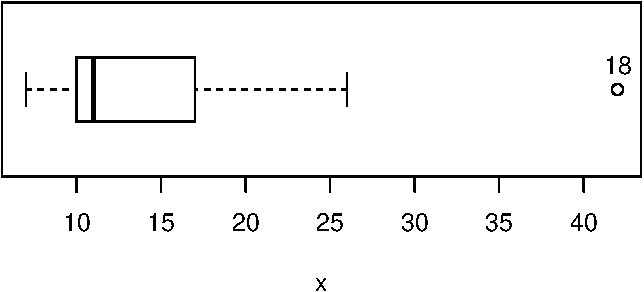
\includegraphics[width=3in]{figuras/chap02_boxplot_x-crop.pdf}
\\ Fonte: Elaborada pelo autor.
\end{center}
\end{figure}


\begin{figure}[h]
\begin{center}
\caption{Boxplot da distribuição da variável $y$}
\label{fig:chap02_boxplot_y-crop}
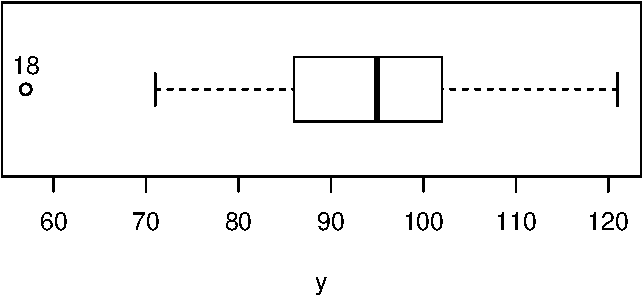
\includegraphics[width=3in]{figuras/chap02_boxplot_y-crop.pdf}
\\ Fonte: Elaborada pelo autor.
\end{center}
\end{figure}

\begin{figure}[h]
\begin{center}
\caption{Diagrama de dispersão com pontos discrepantes destacados}
\label{fig:chap02_simple_scatter}
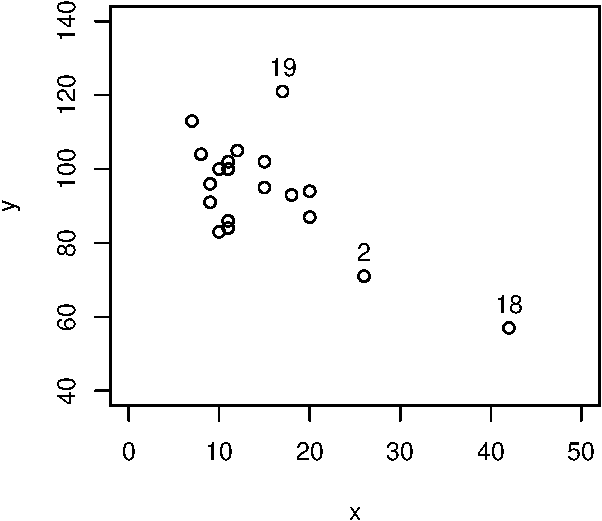
\includegraphics[width=3in]{figuras/chap02_simple_scatter.pdf}
\\ Fonte: Elaborada pelo autor.
\end{center}
\end{figure}

Na Tabela \ref{tab:chap02_estimatives}, temos as estimativas dos parâmetros para o modelo normal e do modelo $t$-Student com os graus de liberdade fixados em $\nu=5$. Como obtemos uma amostra da distribuição \textit{a posteriori} de cada parâmetro em cada distribuição, tomamos como estimativa pontual desses parâmetros a média das respectivas distribuições \textit{a posteriori}. As estimativas dos modelos são parecidas, porém a medida $LPML$ possui um valor maior para o modelo $t$-Student, indicando que este modelo ajusta melhor os dados em relação ao normal.

\begin{table}[h]
\centering
\caption{Estimativas dos parâmetros dos modelos}
\label{tab:chap02_estimatives}
\begin{tabular}{l|cc}
                   & \multicolumn{2}{c}{Modelo}                \\ \cline{2-3} 
Parâmetros         & \multicolumn{1}{c|}{Normal} & $t$-Student \\ \hline 
$\beta_0$          & \multicolumn{1}{c|}{109.82} & 110.42      \\
$\beta_1$          & \multicolumn{1}{c|}{-1.12}  & -1.18       \\
$Var(\varepsilon)$ & \multicolumn{1}{c|}{131.79} & 143.04      \\
$LPML$             & \multicolumn{1}{c|}{-82.99} & -82.05      \\ \hline
\end{tabular}
\\ Fonte: Elaborada pelo autor.
\end{table}

Um alto valor para $CPO_i$ indica um melhor ajuste do modelo à observação $y_i$, enquanto que um baixo valor sugere que $y_i$ é uma observação discrepante e, possivelmente, influente nas estimativas. Na Figura \ref{fig:chap02_cpo}, reportamos $-\log(CPO_i)$ que deixa mais visível as observações discrepantes por terem valores maiores nesta transformação. A observação 19 é a mais discrepante em termos do $CPO$ para ambos modelos, porém o modelo $t$-Student acomoda melhor esta observação. Note também que a observação 18 possui um $CPO$ não muito elevado não sendo apontada como discrepante segundo esse critério. Note que essa observação se encontra perto da reta de regressão estimada, como se vê na Figura \ref{fig:chap02_scatter_w_regs}.

\begin{figure}[h]
\begin{center}
\caption{$-\log(CPO)$ para os modelos normal e $t$-Student}
\label{fig:chap02_cpo}
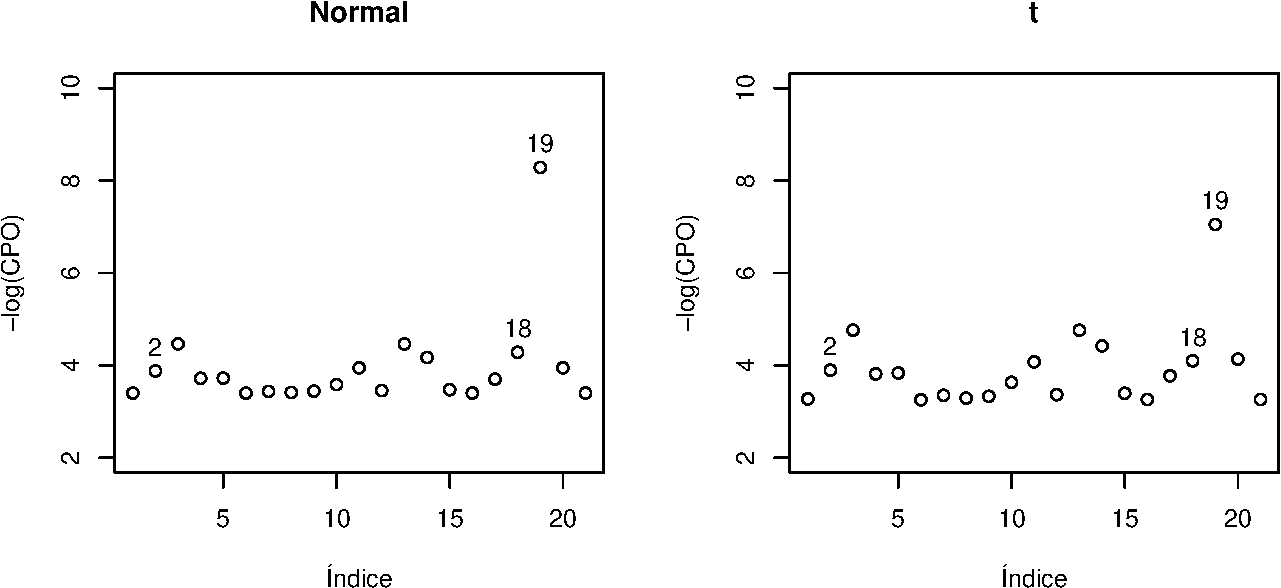
\includegraphics[width=\textwidth]{figuras/chap02_cpo.pdf}
\\ Fonte: Elaborada pelo autor.
\end{center}
\end{figure}

\begin{figure}[h]
\begin{center}
\caption{Diagrama de dispersão com as retas de regressão estimadas}
\label{fig:chap02_scatter_w_regs}
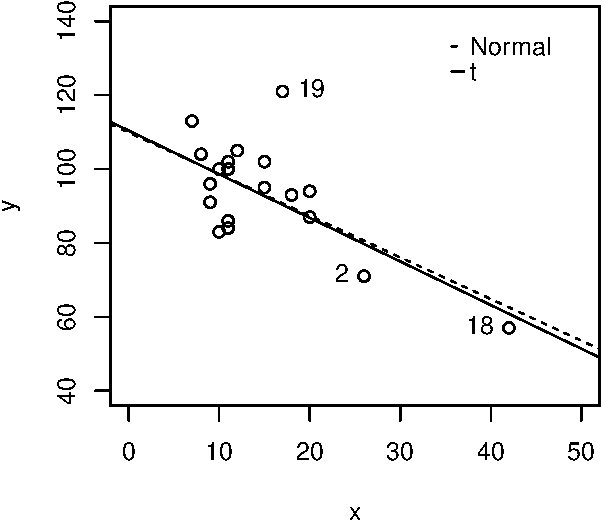
\includegraphics[width=3in]{figuras/chap02_scatter_w_regs-crop.pdf}
\\ Fonte: Elaborada pelo autor.
\end{center}
\end{figure}

Ao analisarmos a influência nas estimativas de forma global, isto é, no vetor $(\betabf,\sigsq)$, verificamos nas Figuras \ref{fig:chap02_l1_global} e \ref{fig:chap02_kl_global} que a observação 18 agora também recebe destaque, considerando ambas medidas de influência global. A observação 18 possui uma forte influência nas estimativas dos modelos enquanto que a observação 19 possui uma influência menor no modelo $t$-Student se compararmos com o modelo normal. Dessa forma, pontos como o 19, de resíduo elevado e mais próximo dos demais, mostram como o modelo $t$-Student é mais robusto que o normal, isto é, menos afetado por observações discrepantes.

Já na influência nas estimativas de forma marginal (em $\betabf$), podemos ver nas Figuras \ref{fig:chap02_l1_marg} e \ref{fig:chap02_kl_marg} que a observação 19 sob o modelo normal possui uma menor influência, indicando que esta observação influencia mais as estimativas de $\sigsq$. Sob o modelo $t$-Student, as observações possuem influências mais parecidas com o caso global. Entre os modelos, o modelo $t$-Student é aquele com as menores medidas de influência para as observações 18 e 19 como podemos verificar na Tabela \ref{tab:chap02_diag}.

\begin{figure}[h]
\begin{center}
\caption{Influência global via norma $L_1$}
\label{fig:chap02_l1_global}
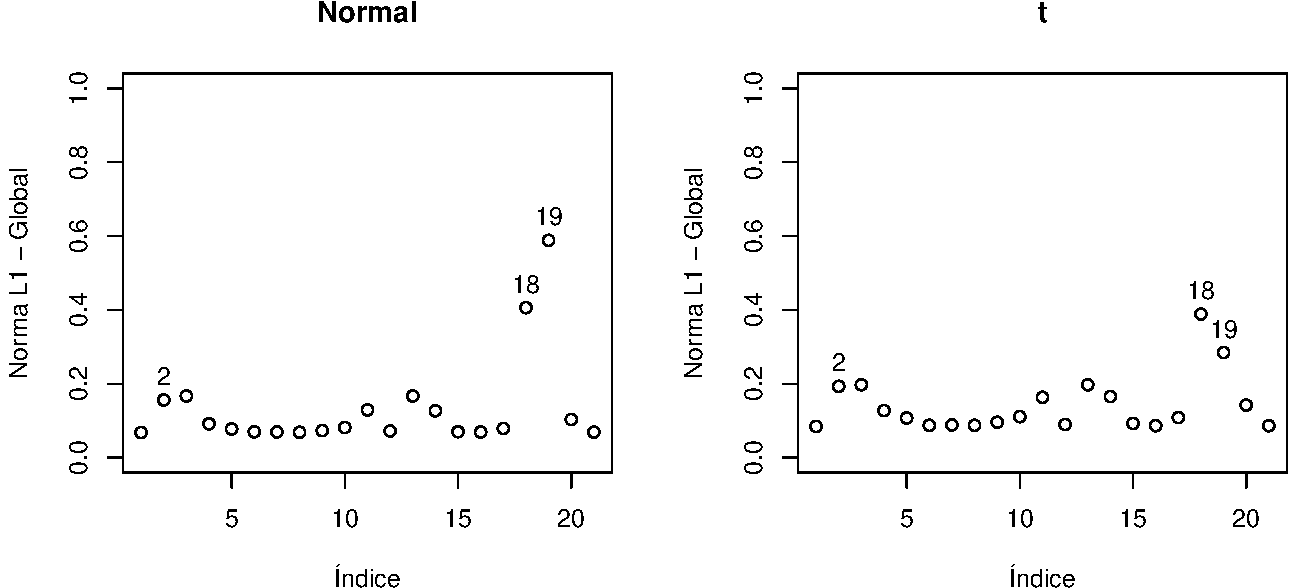
\includegraphics[width=\textwidth]{figuras/chap02_l1_global.pdf}
\\ Fonte: Elaborada pelo autor.
\end{center}
\end{figure}

\begin{figure}[h]
\begin{center}
\caption{Influência global via Kullback-Leibler}
\label{fig:chap02_kl_global}
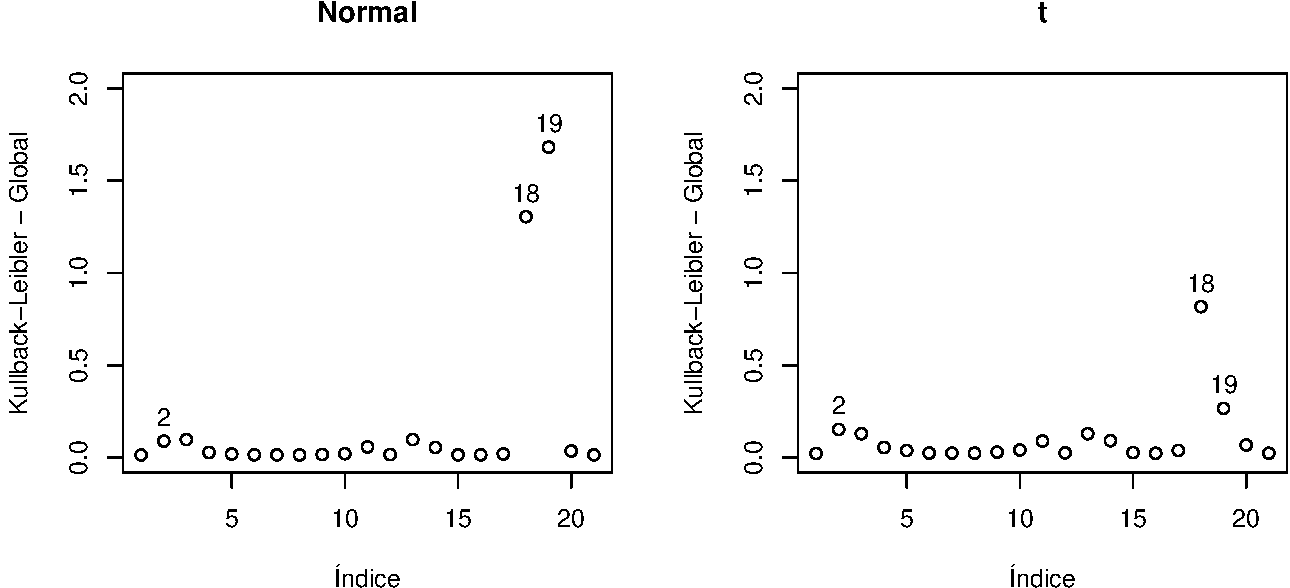
\includegraphics[width=\textwidth]{figuras/chap02_kl_global.pdf}
\\ Fonte: Elaborada pelo autor.
\end{center}
\end{figure}

\begin{figure}[h]
\begin{center}
\caption{Influência marginal em $\betabf$ via norma $L_1$}
\label{fig:chap02_l1_marg}
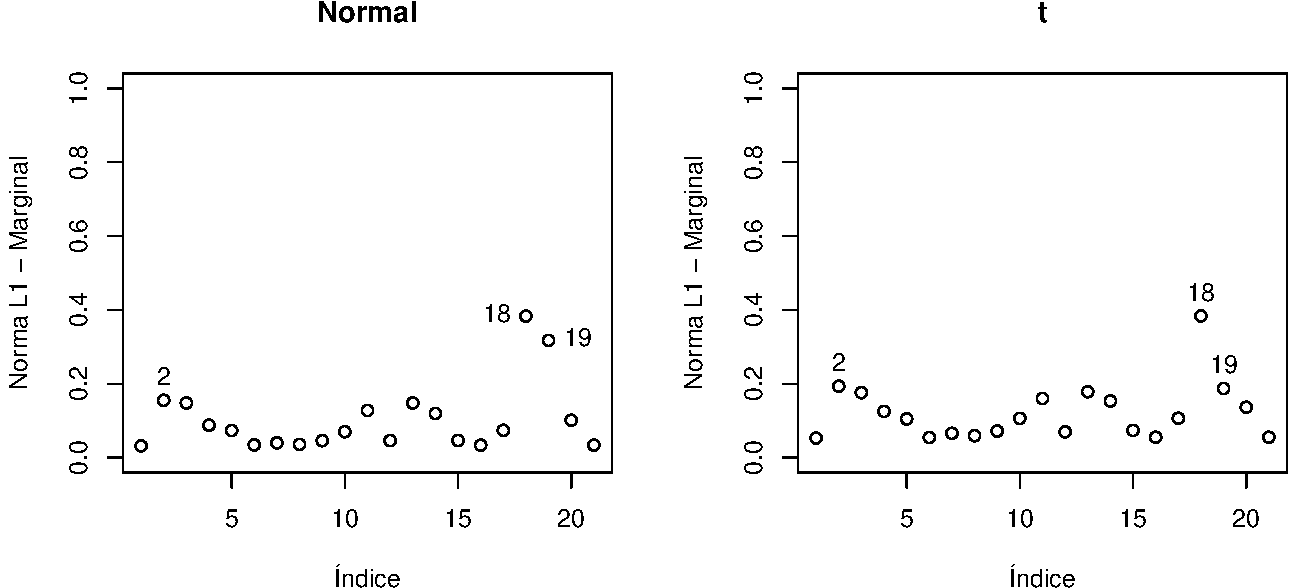
\includegraphics[width=\textwidth]{figuras/chap02_l1_marg.pdf}
\\ Fonte: Elaborada pelo autor.
\end{center}
\end{figure}

\begin{figure}[h]
\begin{center}
\caption{Influência marginal em $\betabf$ via Kullback-Leibler}
\label{fig:chap02_kl_marg}
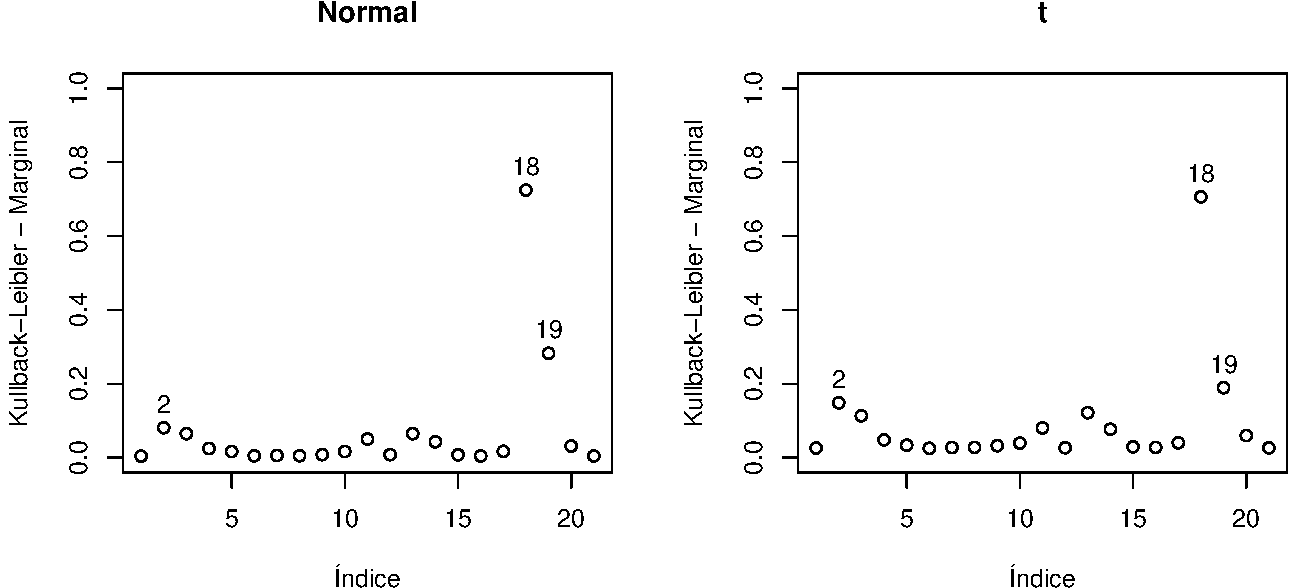
\includegraphics[width=\textwidth]{figuras/chap02_kl_marg.pdf}
\\ Fonte: Elaborada pelo autor.
\end{center}
\end{figure}

\begin{table}[h]
\centering
\caption{Medidas de diagnóstico para as observações 2, 18 e 19}
\label{tab:chap02_diag}
\begin{tabular}{ll|c|c|c|c|cc}
 & Observação & \multicolumn{2}{c|}{2} & \multicolumn{2}{c|}{18} & \multicolumn{2}{c}{19} \\ \hline %\cline{2-8} 
 & Modelo & Normal & t & Normal & t & \multicolumn{1}{c|}{Normal} & t \\ \hline
Medida & $CPO_i$ & 0.0207 & 0.0203 & 0.0138 & 0.0167 & \multicolumn{1}{c|}{0.00025} & 0.00087 \\
 & $L_{1i,(\betabf,\sigma^2)}$ & 0.156 & 0.193 & 0.406 & 0.389 & \multicolumn{1}{c|}{0.588} & 0.285 \\
 & $L_{1i,\betabf}$ & 0.155 & 0.194 & 0.383 & 0.384 & \multicolumn{1}{c|}{0.318} & 0.187 \\
 & $K_{1i,(\betabf,\sigma^2)}$ & 0.09 & 0.153 & 1.305 & 0.818 & \multicolumn{1}{c|}{1.682} & 0.267 \\
 & $K_{1i,\betabf}$ & 0.081 & 0.149 & 0.724 & 0.706 & \multicolumn{1}{c|}{0.283} & 0.189 \\ \hline
\end{tabular}
\\ Fonte: Elaborada pelo autor.
\end{table}
